\subsection{Validation} \label{sec:VandV_rans_uq}

Before the eigenspace perturbation methodology can be applied to flow simulations involving complex geometries, it is essential that the methodology is tested on a range of flow configurations that are often used to validate CFD codes. Continuing to use \cite{computational_fluid_dynamics_committee_guide_1998} as a guide, validation refers to 
\say{The process of determining the degree to which a model is an accurate representation of the real world from the perspective of the intended uses of the model.} In the context of the eigenspace perturbation methodology, validation involves ensuring the predicted uncertainty estimates are a reasonable representation of the uncertainty injected by the turbulence model being used. Flow configurations with either experimental data or high-fidelity simulation data are required to validate the methodology. It should meet the following expectations:

\begin{enumerate}
    \item If there is discrepancy between the RANS simulation predictions and the experimental data, the uncertainty estimates should be large.
    \item If the RANS simulations predictions agree with the experimental data, the uncertainty estimates should be small. 
\end{enumerate}

In an ideal case, if the turbulence model was the only source of uncertainty and error, all the experimental data should lie within the uncertainty estimates from the methodology. In practice, this is rarely the case. Often errors stemming from insufficient numerical discretization or a discrepancy in experimental and simulation conditions, affect the quality of the simulation prediction. 

This section presents results for the uncertainty estimation module for a range of test cases detailed in Table \ref{tab:vandv_cases}. The first two flows are benchmark cases widely used for the testing of turbulence models. They test the ability of the methodology to predict the behavior of highly separated flows. The final four cases are flows of interest to aerospace design. The jet flows test the methodology's performance for shear-layer flows, whereas the airfoil flows test its performance over a range of flow regimes. The SST turbulence model of \cite{sst} was used for all the results. 

\begin{table}
\caption{\label{tab:vandv_cases} Details of testing and validation cases}
\begin{center}
\begin{tabular}{ccc}
Test Case& Rationale& Notes \\\hline
Turbulent flow over a backward facing step& Benchmark flow& 2D, incompressible simulation.\\
Turbulent flow through an asymmetric diffuser& Benchmark flow& 2D, compressible simulation.\\
Jet effluxes from the NASA Acoustic Response Nozzle& Engineering case & 3D, sub-sonic simulation.\\
Cooled Jet via the NASA Seiner Nozzle& Engineering case& 3D, super-sonic simulation.\\
NACA 0012 airfoil at a range of angles of attack& Engineering case& 2D, sub-sonic simulation.\\
Turbulent flow over a three-element High-lift airfoil& Engineering case& 2D, sub-sonic simulation.\\
\end{tabular}
\end{center}
\end{table}

\subsection{Turbulent flow over a backward facing step}

\begin{figure}
    \centering
    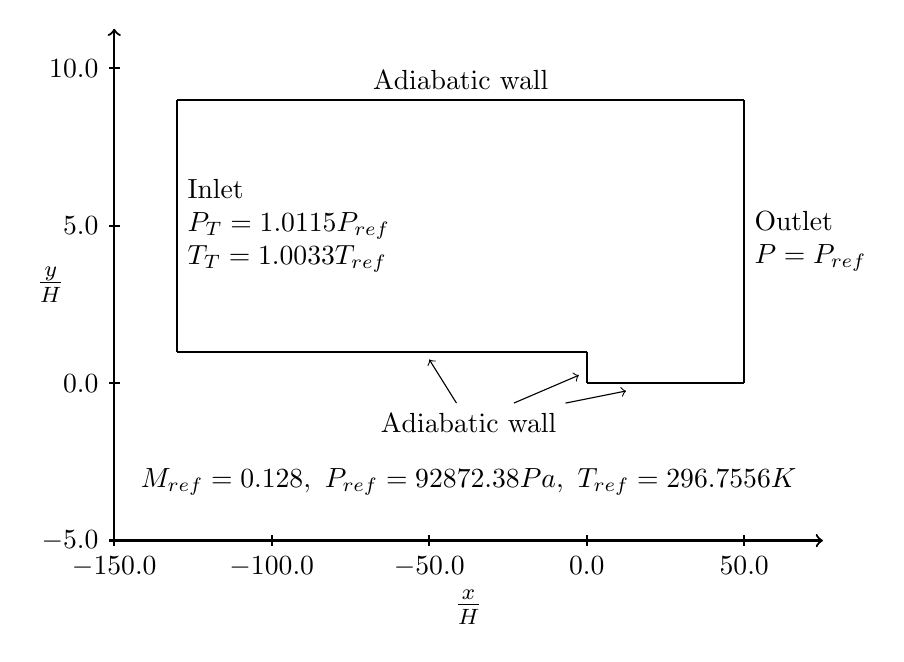
\begin{tikzpicture}

% \draw[step=0.4cm,gray,very thin] (0,0) grid (10,8);
        \draw[thick,->] (0,0) -- node[anchor=north,yshift= -0.5cm,font=\large] {$\frac{x}{H}$} (9,0) ;
        \draw[thick,->] (0,0) -- node[anchor=east,xshift= -0.5cm,font=\large] {$\frac{y}{H}$}(0,6.5) ;
    
        \foreach \x in {0,2,4,6,8}
           \draw [thick](\x cm,2pt) -- (\x cm,-2pt) node[anchor=north] {$\pgfmathparse{\x*25-150}\pgfmathresult$};
        \foreach \y in {0,2,4,6}
            \draw [thick](2pt,\y cm) -- (-2pt,\y cm) node[anchor=east] {$\pgfmathparse{\y*2.5-5}\pgfmathresult$};
        
        \draw[thick] (6,2) -- (8,2) ;
        \draw[thick] (8,2) -- node[anchor=west,align=left] {Outlet\\$P=P_{ref}$} (8,5.6);
        \draw[thick] (8,5.6) -- node[anchor=south] {Adiabatic wall}(0.8,5.6);   
        \draw[thick] (0.8,5.6) -- node[anchor=west,align=left] {Inlet\\$P_T = 1.0115 P_{ref}$\\$T_T = 1.0033 T_{ref}$} (0.8,2.4);   
        \draw[thick] (0.8,2.4) -- (6,2.4);
        \draw[thick] (6,2.4) -- (6,2.0);
        \node (wall) [xshift=4.5cm,yshift=1.5cm] {Adiabatic wall};
        \draw [->](wall) -- (6.5,1.9);
        \draw [->](wall) -- (5.9,2.1);
        \draw [->](wall) -- (4,2.3);
        \node (cond) [xshift=4.5cm,yshift=0.75cm,align=center] {$M_{ref}= 0.128,~P_{ref} = 92872.38 Pa,~T_{ref} = 296.7556 K$};

    \end{tikzpicture}
    \caption{Geometry and simulation conditions for turbulent flow over a backward facing step.}
    \label{fig:backstep_config}
\end{figure}


\begin{figure}
\centering
\includegraphics[width=0.8\textwidth]{code/image_gen/backstep/images/backstep_cf_bot.png}
\caption{Coefficient of friction ($C_f$) over the bottom wall for the flow over a backward facing step. The filled circles mark the experimental data of \cite{driver1985}, the solid line represents the unperturbed RANS simulation and the gray shaded zones are the uncertainty bounds\label{fig:backstep_cf}}
\end{figure}

\begin{figure}
\centering
\includegraphics[width=0.8\textwidth]{code/image_gen/backstep/images/backstep_vel_prof.png}
\caption{Mean velocity profiles for the flow over a backward facing step. The filled circles mark the experimental data of \cite{driver1985}, the solid line represents the unperturbed RANS simulation and the gray shaded zones are the uncertainty bounds\label{fig:backstep_vel_prof}}
\end{figure}

Figure \ref{fig:backstep_config} illustrates the flow geometry and simulation conditions that are used. The inlet and outlet boundary conditions are chosen to yield the correct Mach number $\left ( M_{ref} = 0.128 \right )$ upstream from the step. The figure is scaled by the step height $\left ( H \right ) $. Note that the $x$ and $y$ axes have different scales. This helps in visualizing the geometry since the geometry is $\approx 20\times$ longer in the $x$ direction when compared to the channel height. The channel height, after the step, is $9H$. 

The flow is allowed to fully develop before flowing over the step. The sudden expansion in the channel height results in flow separation and subsequent reattachment downstream from the step. The size of the resulting re-circulation region or the re-attachment length is a key quantity that must be predicted accurately by a turbulence model. Classical two-equation turbulence models under predicted the re-attachment length by 10-25\% \cite{thangam1991}.This occurs due to inaccurate predictions for normal Reynolds stress differences arising from the use of an isotropic eddy viscosity \cite{thangam1991}. This configuration has been investigated experimentally by \cite{driver1985} and their data is used in our investigation.

Fig. \ref{fig:backstep_cf} shows the coefficient of friction ($c_f$) along the bottom wall. The uncertainty estimates are able to account for the discrepancy between model predictions and experimental data at most locations. Fig. \ref{fig:backstep_vel_prof} outlines the axial mean velocity profiles in the flow, after the step. While there is some discrepancy between the unperturbed RANS simulation and the experimental data, the uncertainty intervals are able to account for most of this discrepancy with almost all experimental data points lying in the uncertainty bounds. 

\subsection{Turbulent flow through an asymmetric diffuser}
\begin{figure}
    \centering
    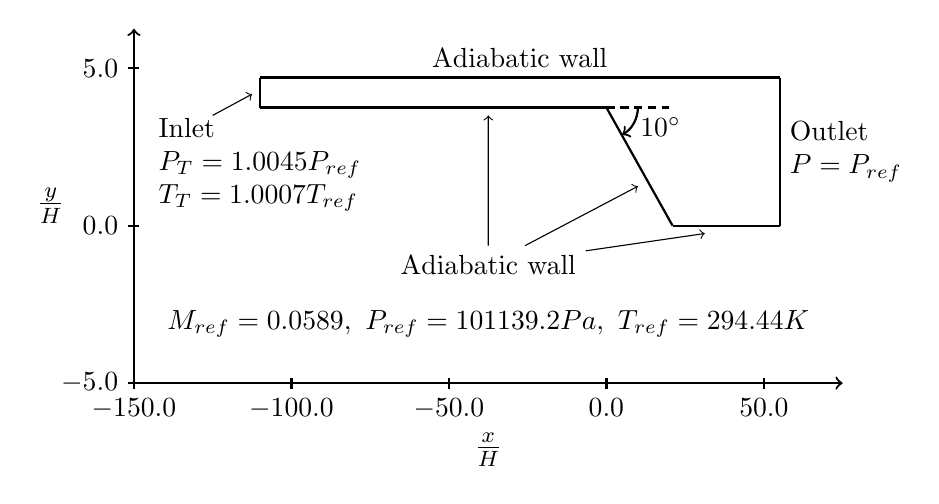
\begin{tikzpicture}

% \draw[step=0.4cm,gray,very thin] (0,0) grid (10,8);
        \draw[thick,->] (0,0) -- node[anchor=north,yshift= -0.5cm,font=\large] {$\frac{x}{H}$} (9,0) ;
        \draw[thick,->] (0,0) -- node[anchor=east,xshift= -0.75cm,font=\large] {$\frac{y}{H}$}(0,4.5) ;

        \foreach \x in {0,2,4,6,8}
           \draw [thick](\x cm,2pt) -- (\x cm,-2pt) node[anchor=north] {$\pgfmathparse{\x*25-150}\pgfmathresult$};
        \foreach \y in {0,2,4}
            \draw [thick](2pt,\y cm) -- (-2pt,\y cm) node[anchor=east] {$\pgfmathparse{\y*2.5-5}\pgfmathresult$};
        
        \draw[thick] (6.84,2) -- (8.2,2) ;
        \draw[thick] (8.2,2) -- node[anchor=west,align=left] {Outlet\\$P=P_{ref}$} (8.2,3.88);
        \draw[thick] (8.2,3.88) -- node[anchor=south] {Adiabatic wall}(1.6,3.88);   
        \draw[thick] (1.6,3.88) -- (1.6,3.5) node (inlet_label) [anchor=north,align=left] {Inlet\\$P_T = 1.0045 P_{ref}$\\$T_T = 1.0007 T_{ref}$};   
        \draw[thick] (1.6,3.5) -- (6.0,3.5);
        \draw [thick, densely dashed] (6,3.5) -- (6.8,3.5);
        \draw [thick, ->] (6.4,3.5) arc (0:-60:.4) node [anchor=west, xshift=0.1cm, yshift=0.1cm](angle_label) {$10^\circ$};
        \draw[thick] (6,3.5) -- (6.84,2.0);
        \node (wall) [xshift=4.5cm,yshift=1.5cm] {Adiabatic wall};
        \draw [->](wall) -- (7.25,1.9);
        \draw [->](wall) -- (6.4,2.5);
        \draw [->](wall) -- (4.5,3.4);
        \draw [->](1.0,3.4) -- (1.5,3.67);
        \node (cond) [xshift=4.5cm,yshift=0.75cm,align=center] {$M_{ref}= 0.0589,~P_{ref} = 101139.2 Pa,~T_{ref} = 294.44 K$};

    \end{tikzpicture}
    \caption{Geometry and simulation conditions for turbulent flow through an asymmetric diffuser.}
    \label{fig:diffuser_config}
\end{figure}

\begin{figure}
\centering
\subfigure[\label{fig:diffuser_cf_top}Coefficient of friction ($C_f$) over the top wall ] %
  {\includegraphics[width=0.8\textwidth]{code/image_gen/diffuser/images/diffuser_cf_top.png}}
\subfigure[\label{fig:diffuser_cf_bot}Coefficient of friction ($C_f$) over the bottom wall ] %
  {\includegraphics[width=0.8\textwidth]{code/image_gen/diffuser/images/diffuser_cf_bot.png}}
\caption{Coefficient of friction ($c_f$) over the top and bottom walls for the flow in an asymmetric diffuser. The filled circles mark the experimental data of \cite{buice}, the solid line represents the unperturbed RANS simulation and the gray shaded zones are the uncertainty bounds.\label{fig:diffuser_cf}}
\end{figure}

Figure \ref{fig:diffuser_config} illustrates the flow geometry and simulation conditions that are used. The flow is allowed to fully develop in the channel leading up to the diffuser. The channel height, $H$, is used to normalize the geometry's length scale. As before, the $x$ and $y$ axes have different scales to make it easier to represent the geometry. This difference in scales greatly exaggerates the angle of the diffuser, which is $10^\circ$ as labeled in Figure \ref{fig:diffuser_config}. The reference pressure, $P_{ref}$, was adjusted to ensure the channel centerline velocity just upstream of the diffuser is $22.6 m/s$. 

Turbulent flow in an asymmetric diffuser has many interesting properties, such as separation over a smooth wall, subsequent reattachment, and redevelopment of the downstream boundary layer, that offer considerable challenges to eddy-viscosity based models. We use the experimental data of \cite{buice}. The data include mean velocities at various stations in the diffuser and skin friction data on the upper and lower walls. 

Fig. \ref{fig:diffuser_cf_top} and \ref{fig:diffuser_cf_bot} exhibit the coefficient of friction ($c_f$) over the top and bottom walls. While there is considerable discrepancy between the RANS prediction and the experimental data, the uncertainty intervals are able to account for a substantial proportion of this discrepancy. Most of the experimental data points lie inside the uncertainty intervals. Fig. \ref{fig:diffuser_vel_prof} exhibits the axial mean velocity profiles at a range of locations along the diffuser. The uncertainty bounds encompass most of the experimental data points, including in the region of flow separation. 

\begin{figure}
\centering
\includegraphics[width=0.8\textwidth]{code/image_gen/diffuser/images/diffuser_vel_prof.png}
\caption{Mean velocity profiles for the flow in the axisymmetric diffuser. The filled circles mark the experimental data of \cite{buice}, the solid line represents the unperturbed RANS simulation and the gray shaded zones are the uncertainty bounds\label{fig:diffuser_vel_prof}}
\end{figure}

\subsection{Jet efflux of the NASA Acoustic Response Nozzle}
\begin{figure}
    \centering
    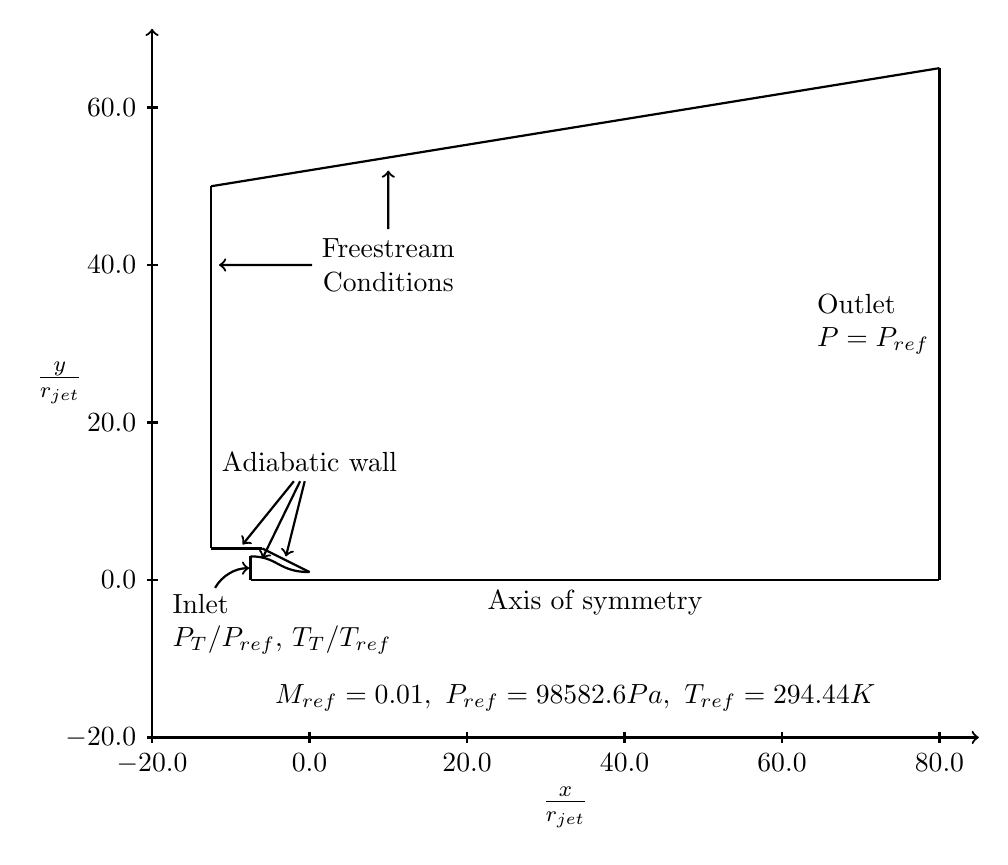
\begin{tikzpicture}

% \draw[step=0.4cm,gray,very thin] (0,0) grid (10,8);
        \draw[thick,->] (0,0) -- node[anchor=north,yshift= -0.5cm,font=\large] {$\frac{x}{r_{jet}}$} (10.5,0) ;
        \draw[thick,->] (0,0) -- node[anchor=east,xshift= -0.75cm,font=\large] {$\frac{y}{r_{jet}}$}(0,9.0) ;

        \foreach \x in {0,2,4,6,8,10}
           \draw [thick](\x cm,2pt) -- (\x cm,-2pt) node[anchor=north] {$\pgfmathparse{\x*10-20}\pgfmathresult$};
        \foreach \y in {0,2,4,6,8}
            \draw [thick](2pt,\y cm) -- (-2pt,\y cm) node[anchor=east] {$\pgfmathparse{\y*10-20}\pgfmathresult$};
        
        \draw[thick] (1.25,2) -- node[anchor=north,align=center] {Axis of symmetry} (10,2) ;
        \draw[thick] (10,2) -- node[anchor=east,align=left] {Outlet\\$P=P_{ref}$} (10,8.5);
        \draw[thick] (10,8.5) -- (0.75,7);   
        \draw[thick] (0.75,7) -- (0.75,2.4) ;   
        \draw[thick] (0.75,2.4) -- (1.4,2.4);
        \draw[thick] (1.4,2.4) -- (2,2.1);
        \draw[thick] (2,2.1) .. controls (1.6,2.1) and (1.6,2.3) .. (1.25,2.3);
        \draw[thick] (1.25,2.3) -- (1.25,2) node (inlet_label) [anchor=north,align=left,xshift=.4cm,yshift=-0.05cm] {Inlet\\$P_T/P_{ref}$, $T_T/T_{ref}$};
        \node (freestream_label)[xshift=3cm,yshift=6cm,align=center]{Freestream\\Conditions};
        \draw [->,thick](freestream_label) -- (3.0,7.2);
        \draw [->,thick](freestream_label) -- (.85,6);
        \draw [->,thick] (0.8,1.9)  arc (150:90:.5cm);
        \node (cond) [xshift=5.375cm,yshift=0.5cm,align=center] {$M_{ref}= 0.01,~P_{ref} = 98582.6 Pa,~T_{ref} = 294.44 K$};
        \node (wall_label) [xshift=2cm,yshift=3.5cm,align=center] {Adiabatic wall};
        \draw [->,thick] (wall_label) -- (1.15,2.45);
        \draw [->,thick] (wall_label) -- (1.7,2.3);
        \draw [->,thick] (wall_label) -- (1.4,2.27);

    \end{tikzpicture}
    \caption{Geometry and boundary conditions for jet efflux from the NASA Acoustic Response Nozzle.}
    \label{fig:arn_config}
\end{figure}



Reliable predictions of turbulent jets exhausting from aircraft nozzles are essential for a variety of aerospace design applications. However, these exhaust jets involve a multitude of complications such as the interaction of the jet efflux and the ambient, complicated nozzle geometries, compressibility effects, under or over-expanded flows, etc. These pose significant challenges to eddy-viscosity based models. As an illustration, lets focus on the mixing between the jet and the ambient fluid. In the vicinity of the nozzle exit, RANS models predict a significantly lower rate of jet mixing as compared with high-fidelity data. Farther downstream of the jet potential core, RANS models predict the far-field mixing rate to become substantially higher than is observed in experiments. Similarly, the fidelity of RANS predictions is highly inconsistent, having higher fidelity for cold jets than heated, for axi-symmetric than non-axi-symmetric geometries, varying significantly over different quantities of interest, etc. 

In this test case, we investigate sub-sonic jets from the NASA Acoustic Response Nozzle. This has been studied experimentally by \cite{nasajet} and extensive Particle Image Velocimetry data are available. The PIV data set was generated at the Small Hot Jet Acoustic Rig at the NASA Glenn Research Center. The tests were repeated on numerous instances during 2001-2007 with varying PIV configurations. In addition to a robust mean, this corpus provides insight into the data uncertainty. The raw data set consists of over 23,000 velocity fields available for statistical analysis at each location. The researchers have also shared a final consensus dataset, with the averaged mean over the raw data along with the standard deviations over the measurements at each point, termed as error bars in the data set by \cite{nasajet}. This data uncertainty attempts to account for any statistical bias and random errors in the measurements arising from PIV calibration, image analysis procedure, rig flow instrumentation, small errors in the instantaneous measurements, the size and number of ensembles used, etc. 

Figure \ref{fig:arn_config} represents the geometry and flow conditions that are simulated. The ambient flow speed is kept very low, at $M = 0.01$. The inlet total pressure and temperature ratios are set according to the specific case that is being run. Outlined here are the results for different subsonic jet conditions. The inlet ratios and Mach number at the jet throat are detailed in Table 2.


\begin{table}
\caption{\label{tab:table2} Reference conditions for subsonic jet flow cases considered}
%\begin{ruledtabular}
\begin{center}
\begin{tabular}{ccccc}
Test Case & Classification& $Ma$& ${T_T}/{T_{ref}}$& ${P_T}/{P_{ref}}$\\\hline
Case I  & heated, perfectly expanded & 0.376 & 1.764 & 1.102\\
Case II & cooled, perfectly expanded & 0.513 & 0.950 & 1.197\\
\end{tabular}
\end{center}
%\end{ruledtabular}
\end{table}

\begin{figure}
\centering
\subfigure[\label{fig:arn_sp23_center_vel}Axial velocity variation over the centerline] %
  {\includegraphics[trim=25 0 25 0, clip,width=\textwidth]{code/image_gen/arn/sp23/images/arn_sp23_center_vel.png}}
\subfigure[\label{fig:arn_sp23_vel_prof}Mean axial velocity profiles in the wake, delineated at $x/D_{jet}= 4,8, 12$ and $16$] %
  {\includegraphics[trim=25 0 25 0, clip,width=\textwidth]{code/image_gen/arn/sp23/images/arn_sp23_vel_prof.png}}
 \subfigure[\label{fig:arn_sp23_k_prof}Turbulence kinetic energy ($k$) profiles in the wake, delineated at $x/D_{jet}= 4,8, 12$ and $16$] %
  {\includegraphics[trim=25 0 25 0, clip,width=\textwidth]{code/image_gen/arn/sp23/images/arn_sp23_k_prof.png}}
\caption{Comparison of experimental data and RANS simulation data for Case I of flow through the NASA Acoustic Response Nozzle. The filled circles mark the mean PIV data of \cite{nasajet}, the error bars represent the $\pm 1-\sigma$ variance in the recorded data, the solid line represents the unperturbed RANS simulation and the gray shaded zones are the uncertainty estimates.\label{fig:arn_sp23}}
\end{figure}

\begin{figure}
\centering
\subfigure[\label{fig:arn_sp3_center_vel}Axial velocity variation over the centerline] %
  {\includegraphics[trim=25 0 25 0, clip,width=\textwidth]{code/image_gen/arn/sp3/images/arn_sp3_center_vel.png}}
\subfigure[\label{fig:arn_sp3_vel_prof}Mean axial velocity profiles in the wake, delineated at $x/D_{jet}= 4,8, 12$ and $16$] %
  {\includegraphics[trim=25 0 25 0, clip,width=\textwidth]{code/image_gen/arn/sp3/images/arn_sp3_vel_prof.png}}
 \subfigure[\label{fig:arn_sp3_k_prof}Turbulence kinetic energy ($k$) profiles in the wake, delineated at $x/D_{jet}= 4,8, 12$ and $16$] %
  {\includegraphics[trim=25 0 25 0, clip,width=\textwidth]{code/image_gen/arn/sp3/images/arn_sp3_k_prof.png}}
\caption{Comparison of experimental data and RANS simulation data for Case II of flow through the NASA Acoustic Response Nozzle. The filled circles mark the mean PIV data of \cite{nasajet}, the error bars represent the $\pm 1-\sigma$ variance in the recorded data, the solid line represents the unperturbed RANS simulation and the gray shaded zones are the uncertainty estimates.\label{fig:arn_sp3}}
\end{figure}


\begin{figure}
\includegraphics[width=1.05\textwidth]{Figure13.pdf}
\caption{Mean axial velocity profiles in the NASA ARN exhaust , delineated at $x/D_j= 4,8,12$ and $16$\label{fig:fig5}}
\end{figure}

Figure \ref{fig:arn_sp23} and Figure \ref{fig:arn_sp3} present the results for Case I and II respectively. The mean experimental data is represented by the solid black dots and the associated error bars represent the reported standard deviation of the PIV data. The solid black line represents the baseline result using the unperturbed SST turbulence model and the gray area is the uncertainty estimated by the eigenspace perturbation methodology. The first subplot, Figure \ref{fig:arn_sp23_center_vel} and Figure \ref{fig:arn_sp3_center_vel}, plots the normalized axial velocity along the jet centerline. The centerline velocity at the jet exit, $U_{jet}$ is used as the normalizing factor. The second subplot, Figure \ref{fig:arn_sp23_vel_prof} and Figure \ref{fig:arn_sp3_vel_prof}, shows the normalized axial velocity in the jet wake at four different downstream locations: $x/D_{jet}= 4, 8, 12$, and $16$. The last subplot, Figure \ref{fig:arn_sp23_k_prof} and Figure \ref{fig:arn_sp3_k_prof}, plot the normalized turbulent kinetic energy in the jet wake at the same downstream locations. 

The differences in the solid black line and black dots shows that the baseline turbulence model has great difficulty in accurately capturing the flow physics in the jet wake.  The uncertainty estimates, represented by the grey areas, are able to account for a significant proportion of the discrepancy between the RANS simulations and the high-fidelity experimental data. If the experimental data points themselves don't lie within the grey area, there is a non-trivial intersection between the error bars and the grey area. 

\subsection{Heated Jet through the NASA Seiner Nozzle}


\begin{figure}
\subfigure[\label{fig:fig7a} Mach number variation over the centerline] %
  {\includegraphics[width=0.5\textwidth]{Figure14a.pdf}}
\subfigure[\label{fig:fig7b}Pressure variation over the centerline] %
  {\includegraphics[width=0.5\textwidth]{Figure14b.pdf}}
\caption{Variation in Quantities of Interest over the jet centerline for the cooled supersonic jet \cite{seiner}.}
\end{figure}

In this test case, we transition from sub-sonic to super-sonic jets. Herein, we replicate the experiment configuration of \cite{seiner}. The experiment was conducted on an axisymmetric, convergent-divergent nozzle with diameter $9.144 cm$. The jet exhausted into a quiescent ambient, with  $Ma=2.0$ and Reynolds number $1.3 \times 10^6$. Fig. \ref{fig:fig7a} and \ref{fig:fig7b} outline the variation in the Mach number and pressure along the jet centerline. Fig. \ref{fig:fig7a} indicates that the extent of the jet potential core is over predicted by the RANS model. The turbulence model also over predicts the spreading rate of the jet. This indicates a predicted rate of mixing that is higher than is suggested by the experimental data. However, the uncertainty bounds are able to account for most of the discrepancy in the length of the potential core and the ensuing mixing rate, with almost all the experimental data points lying inside the bounds. 

\subsection{NACA 0012 airfoil at a range of angles of attack}
In this test case, we consider the flow over a NACA 0012 airfoil at a range of angles of attack, varying from 0$^{\circ}$ to 20$^{\circ}$. This design was chosen specifically due to its adoption in the industry. These include in conventional aircraft for instance the wing tips of the Cessna 140A, 207; helicopter designs such as the inboard and outboard blades of the Aerospatiale AS365, Boeing 600N, Lockheed 475; in addition to numerous horizontal and vertical axis wind turbines. The Reynolds number for the simulations is $6\times 10^6$. The flow is sub-sonic with $Ma=0.15$. The experimental data \cite{ladson1988} report the coefficient of lift ($C_L$) and the surface pressure coefficient ($C_P$) for different angles of attack. 

\begin{figure}
\center
\includegraphics[width=0.7\textwidth]{suthesis/images/L6_ls_cl_vs_alpha_uq.png}
\caption{Variation in the coefficient of lift $C_L$ with the angle of attack $\alpha$\label{fig:naca0012_cl_vs_alpha}}
\end{figure}

In Fig \ref{fig:naca0012_cl_vs_alpha}, we outline the variation in the coefficient of lift with the angle of attack $\alpha$. At low angles of attack, there is almost no discernible difference between the RANS predictions and the experimental data. Accordingly, here the uncertainty bounds are negligible. At higher angles of attack closer to stall, there is substantial discrepancy between the RANS predictions and the high fidelity data. For these values of $\alpha$, the uncertainty bounds are substantial as well. At all values of $\alpha$, the uncertainty bounds envelope the experimental data. 

\begin{figure}
\center
\subfigure[\label{fig:naca0012_cpu_10aoa} Coefficient of pressure variation over the upper surface of the airfoil at $\alpha=10^{\circ}$] %
  {\includegraphics[width=1.0\textwidth]{suthesis/images/L6_ls_10aoa_cpu.png}}
\subfigure[\label{fig:naca0012_cpu_15aoa}Coefficient of pressure variation over the upper surface of the airfoil at $\alpha=15^{\circ}$] %
  {\includegraphics[width=1.0\textwidth]{suthesis/images/L6_ls_15aoa_cpu.png}}
\caption{Variation in coefficient of pressure over the airfoil at different angles of attack.}
\end{figure}

Fig. \ref{fig:naca0012_cpu_10aoa} and \ref{fig:naca0012_cpu_15aoa} outline the variation in the coefficient of pressure ($c_p$) variation along the upper surface of the airfoil at angles of attack $\alpha=10^{\circ}$ and $15^{\circ}$ respectively. Away from the stall at $\alpha=10^{\circ}$, the RANS predictions are in good agreement with the experimental data. Accordingly, the uncertainty bounds are negligibly small. At $\alpha=15^{\circ}$, there is significant discrepancy between the RANS predictions and the experimental data. Here, the uncertainty bounds are sizable and envelope the experimental data. For instance, in Fig \ref{fig:naca0012_cpu_15aoa}, there is substantial discrepancy between the experimental data and RANS predictions in the neighborhood of $x/c=0$. However, the uncertainty estimates are able to account for this discrepancy and all the experimental data points intersect the shaded interval estimates.

\subsection{Turbulent flow over a three-element High-lift airfoil}

In this test case, we investigate the turbulent flow over a McDonnell Douglas Aerospace (MDA) single-flap, three-element airfoil. The flap rigging used corresponds to the 30P/30N designated by MDA. The results correspond to the case with Mach number, $Ma=0.2$; Reynolds number, $Re=5 \times 10^6$ with an angle of attack of $\alpha=8^{\circ}$. We use the experimental data of \cite{chin1993}. 

We outline this case as a test against the false positive. In cases where there is significant discrepancy in the RANS predictions, the uncertainty bounds should exhibit the same. However, in cases where the RANS predictions are accurate, having spurious uncertainty bounds that are significant in their extent would be misleading and would correspond to a false positive. \cite{klausmeyer1997} have tested this flow case for a range of RANS models and have found the RANS predictions to be accurate. In such a scenario, ideally, we would expect the uncertainty bounds to be negligible at most locations along the airfoil sections. Fig. \ref{fig:30p30n} outlines the distribution of the coefficient of pressure ($C_p$) on the surfaces of the different sections. The discrepancy between the RANS predictions and the experimental data is very small over the main element and the flap of the airfoil. Accordingly, the uncertainty bounds are negligibly small over these zones. The upper surface of the slat exhibits an appreciable amount of discrepancy between RANS predictions and the high-fidelity data. The uncertainty bounds over this surface are substantial and are able to envelope the experimental data.   



\begin{figure}
\center
\includegraphics[width=0.8\textwidth]{suthesis/images/30p30n_5p5aoa_cp.png}
\caption{Pressure coefficient for the 30P30N configuration\label{fig:30p30n}}
\end{figure}